\chapter{Algoritmos cuánticos}
\label{chapter6}

En este capítulo vamos a embarcarnos en un rápido viaje por el mundo de los algoritmos cuánticos. En primer lugar, exploraremos en profundidad el ya mencionado algoritmo de Deutsch-Jozsa, la prueba matemática de su correcto funcionamiento, su implementación y su código en \textit{Python} y \textit{Qiskit} (disponible en el apéndice~\ref{ap:ap1}, sección~\ref{sec:seca3}). Además,  aprovecharemos la oportunidad que nos da IBM para ejecutar código \textit{Qiskit} en un ordenador cuántico real para comparar los resultados con los obtenidos por nuestro simulador. Por último hablaremos brevemente de algunos de los algoritmos cuánticos más importantes.

\section{Algoritmo de Deutsch-Jozsa}
\label{sec:sec61}

En la sección~\ref{sec:sec11} ya mencionamos este algoritmo. Pese a que el problema que plantea es muy concreto y no es realmente útil, refleja muy bien el poder que puede alcanzar la computación cuántica. Además, como veremos, se trata de un algoritmo determinista y esto nos va a ayudar a reflejar el error cometido por una máquina cuántica real a causa del {\it ruido}, problema mencionado brevemente en la sección~\ref{sec:sec51} cuando hablábamos de \textit{Qiskit Ignis}.

El problema que soluciona este algoritmo se describe así. Sea $\function{f}{\{0,1\}^n}{\{0,1\}}$ una función que cumple una de las dos siguientes condiciones:
\begin{enumerate}
\item $f$ es constante.
\item $f$ es balanceada, es decir, los cardinales de los dos conjuntos $\{x\in{\{0,1\}^n}:f(x)=0\}$ y $\{x\in{\{0,1\}^n}:f(x)=1\}$ son iguales.
\end{enumerate}

Tenemos que determinar qué condición,  de las dos anteriores, verifica $f$. Un algoritmo clásico para la resolución de este problema tendría que hacer, en el caso peor, $2^{n-1}+1$ comprobaciones. El algoritmo de Deutsch-Jozsa sólo requiere de una evaluación. El algoritmo comienza con una preparación similar a la usada por el paralelismo cuántico de la sección~\ref{sec:sec49}. Preparamos $n+1$ qubits, los primeros $n$ en estado $\ket0$ y el último en estado $\ket1$. Tras esto aplicamos una puerta \textit{Hadamard} a cada uno de los $n+1$ qubits obteniendo el estado
\[\dfrac{1}{\sqrt{2^{n+1}}}\sum_{k=0}^{2^n-1}\ket k(\ket0 -\ket1)\]

Ahora aplicamos la transformación $U_f$ que implementa de manera cuántica la función~$f$. En este caso, recordemos que se verifica que $U_f\ket{x,y}=\ket{x,f(x)\oplus y}$, donde $x\in\{0,1\}^n$ e $y\in\{0,1\}$. Por linealidad, aplicando $U_f$ sobre el estado anterior, se obtiene
\[
\begin{split}
\dfrac{1}{\sqrt{2^{n+1}}}U_f\left(\sum_{k=0}^{2^n-1}\ket k(\ket0 -\ket1)\right)&=\dfrac{1}{\sqrt{2^{n+1}}}\sum_{k=0}^{2^n-1}\ket k(\ket{f(k)} -\ket{1\oplus f(k)})\\
&=\dfrac{1}{\sqrt{2^{n+1}}}\sum_{k=0}^{2^n-1}(-1)^{f(k)}\ket k(\ket0 -\ket1)\\
\end{split}
\]

Llegados a este punto podemos prescindir del estado del último qubit y limitarnos al sistema que conforman los primeros $n$ cuyo estado es
\[\dfrac{1}{\sqrt{2^n}}\sum_{k=0}^{2^n-1}(-1)^{f(k)}\ket k\]
%
y aplicamos a estos $n$ qubits de nuevo una puerta de \textit{Hadamard} a cada uno. Conseguimos así:
\[
\begin{split}
&\dfrac{1}{\sqrt{2^n}}\sum_{k=0}^{2^n-1}(-1)^{f(k)}H^{\otimes n}\ket k\\
&=\dfrac{1}{\sqrt{2^n}}\sum_{k_1,...,k_n\in\{0,1\}}(-1)^{f(k_1,...,k_n)}H^{\otimes n}\ket{k_1,...,k_n}\\
&=\dfrac{1}{\sqrt{2^n}}\sum_{k_1,...,k_n\in\{0,1\}}(-1)^{f(k_1,...,k_n)}H\ket{k_1}\otimes\hdots\otimes H\ket{k_n}\\
&=\dfrac{1}{\sqrt{2^n}}\sum_{k_1,...,k_n\in\{0,1\}}(-1)^{f(k_1,...,k_n)}\tfrac{1}{\sqrt{2}}\sum_{z_1\in\{0,1\}}(-1)^{k_1z_1}\ket{z_1}\otimes\hdots\otimes \tfrac{1}{\sqrt{2}}\sum_{z_n\in\{0,1\}}(-1)^{k_nz_n}\ket{z_n}\\
&=\dfrac{1}{\sqrt{2^n}}\sum_{k_1,...,k_n\in\{0,1\}}(-1)^{f(k_1,...,k_n)}\dfrac{1}{\sqrt{2^n}}\sum_{z_1,...,z_n\in\{0,1\}}(-1)^{k_1z_1+\hdots+k_nz_n}\ket{z_1,...,z_n}\\
&=\dfrac{1}{2^n}\sum_{z=0}^{2^n-1}\left(\sum_{k=0}^{2^n-1}(-1)^{f(k)}(-1)^{k*z}\right)\ket{z}\textrm{, donde }k*z=\sum_{i=1}^nk_iz_i
\end{split}
\]

Tras la aplicación de $H^{\otimes n}$, lo último que vamos a hacer es realizar una medición de los~$n$ primeros qubits. En el caso del estado $\ket0^{\otimes n}$, la probabilidad de su obtención viene dada por
\begin{equation}
\label{eq:eq61}
\left|\dfrac{1}{2^n}\sum_{k=0}^{2^n-1}(-1)^{f(k)}\right|^2
\end{equation}

Si $f$ es constante, entonces el sumatorio de la ecuación~\ref{eq:eq61} valdrá $\pm2^n$ según si $f$ es $0$ o $1$. En cualquier caso, la probabilidad de obtener $\ket0^{\otimes n}$ será total. En caso de que $f$ sea balanceada, el sumatorio quedará anulado y por tanto la probabilidad de obtener $\ket0^{\otimes n}$ será 0. Hemos construido así un algoritmo cuántico determinista que soluciona el problema a tratar. En la figura~\ref{fig:fig61} podemos ver el circuito que refleja todas las puertas aplicadas.

\begin{figure}[t]
\[\Qcircuit @C=1em @R=.7em {
\lstick{\ket{0}} & {/^n} \qw & \gate{H^{\otimes n}} & \qw &\multigate{1}{U_f}&\qw& \gate{H^{\otimes n}} & \qw & \meter & \qw \\
\lstick{\ket{1}} & \qw & \gate{H} & \qw & \ghost{U_f}      &\qw& \qw      & \qw & \qw    & \qw}\]
\caption{Circuito de una implementación de Deutsch-Jozsa.}
\label{fig:fig61}
\end{figure}

Vamos a experimentar con este algoritmo. Hemos preparado una clase en \textit{Qiskit}, con ayuda de \textit{Python}, cuyo código está incluido en la sección~\ref{sec:seca3}. Genera un circuito del número de qubits deseado e incluye métodos para ejecutar dicho circuito, obtención de resultados y dos ejemplos de $U_f$, entre otros. El primer ejemplo de $U_f$ que incluimos es la función constante $f\equiv1$ cuya implementación cuántica es tan sencilla como aplicar una puerta $X$ al qubit de salida (el último). El segundo se corresponde con la función $f(x_1,...)=1$ si $x_1=1$ y $0$ en otro caso. Se implementa mediante una simple puerta C$_\textrm{not}$ usando como control el primer qubit y como objetivo el de salida. Independientemente de la dimensión del espacio de entrada, esta función es balanceada. Ejecutaremos ambos ejemplos sobre un simulador y sobre una máquina cuántica real un total de 1024 veces en cada uno de ellos y compararemos los resultados. Estableceremos el tamaño del circuito en 5 qubits (por tanto, la función~$f$ que evaluamos será del tipo $\function{f}{\{0,1\}^4}{\{0,1\}}$). La función balanceada se define entonces como
\[f_1(x_1,x_2,x_3,x_4)=\left\{\begin{matrix}1\textrm{ si } x_1=1\\0\textrm{ si } x_1=0\end{matrix}\right.\]
%
y la puerta $U_f$ viene dada por una puerta C$_\textrm{not}$, usando como control el primer qubit y como objetivo el quinto. Para ejecutar el algoritmo en simulador hacemos uso de la clase que por defecto se ha programado para usar \textit{Qasm simulator} de \textit{Qiskit Aer}, ejecutando el código de la figura~\ref{code:code62}, que crea el circuito, lo ejecuta 1024 veces en dicho simulador e imprime el histograma de la figura~\ref{fig:fig64}.

\begin{figure}[t]
\begin{lstlisting}[language=Python]
from qiskit.visualization import plot_histogram
D = DeutschJozsa()
D.create_circuit(DeutschJozsa.uf_balanced)
D.run(shots = 1024)
plot_histogram(D.get_counts())
\end{lstlisting}
\caption{Código \textit{Python} para ejecutar Deutsch-Jozsa sobre una función balanceada en simulador con ayuda de la clase \textit{DeutschJozsa}.}
\label{code:code62}
\end{figure}

En el caso de querer ejecutarlo en una máquina cuántica de IBM debemos seleccionar un \textit{backend}  como el que presentamos en la figura~\ref{code:code63}. La primera instrucción solicita la máquina cuántica menos ocupada, de al menos 5 qubits y que esté operativa. El resto del código es análogo al anterior e imprime el histograma de la figura~\ref{fig:fig65}.

\begin{figure}[tb!]
\begin{lstlisting}[language=Python]
from qiskit.providers.ibmq import least_busy
backend = least_busy(provider.backends(filters=lambda b: b.configuration().n_qubits >= 5 and not b.configuration().simulator and b.status().operational==True))
D = DeutschJozsa()
D.create_circuit(DeutschJozsa.uf_balanced)
D.run(backend=backend, shots = 1024)
plot_histogram(D.get_counts())
\end{lstlisting}
\caption{Código \textit{Python} para ejecutar Deutsch-Jozsa sobre una función balanceada en computador cuántico con ayuda de la clase \textit{DeutschJozsa}.}
\label{code:code63}
\end{figure}

\begin{figure}[tb!]
    \centering
    \begin{minipage}{0.45\textwidth}
        \centering
        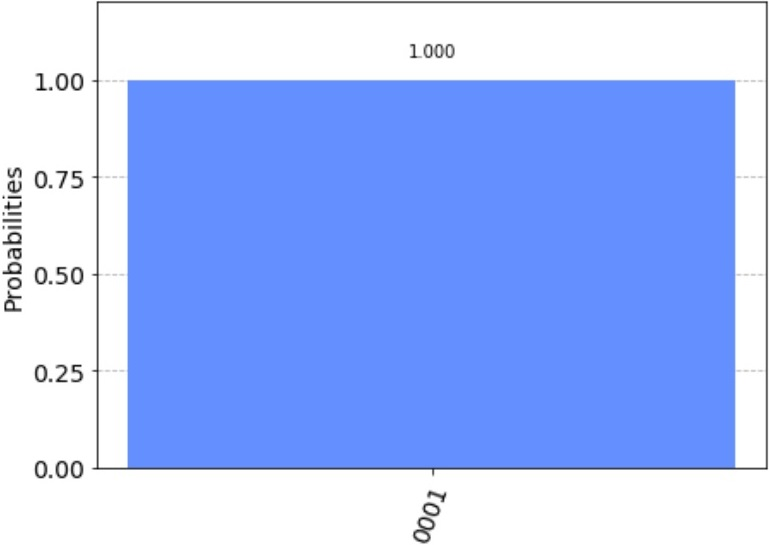
\includegraphics[width=1\textwidth]{images/simulator_balanced}
        \caption{Resultados con función balanceada en simulador.}
        \label{fig:fig64}
    \end{minipage}\hfill
    \begin{minipage}{0.45\textwidth}
        \centering
        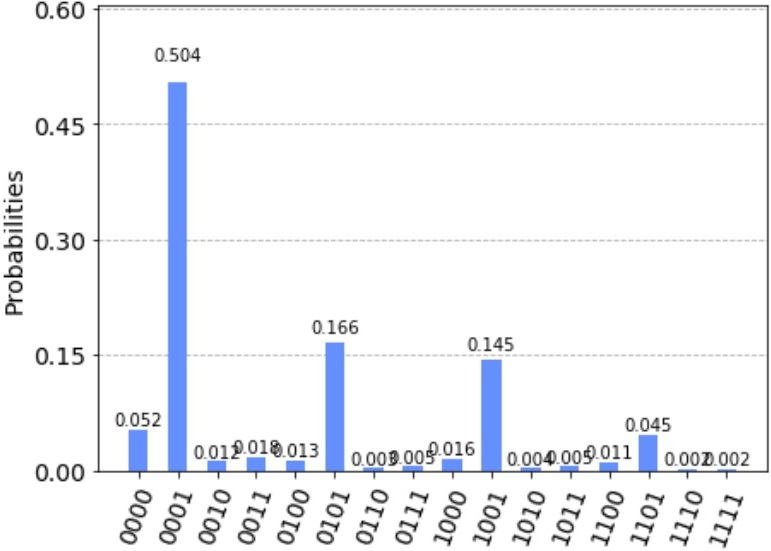
\includegraphics[width=1\textwidth]{images/ibmq_balanced}
        \caption{Resultados con función balanceada en ordenador cuántico de IBM.}
        \label{fig:fig65}
    \end{minipage}
\end{figure}

De acuerdo a los resultados mostrados en los histogramas de las figuras \ref{fig:fig64} y \ref{fig:fig65}, en el caso del simulador se obtiene un 100\% de las veces el estado $\ket{0001}$ que, en efecto, es distinto de $\ket{0000}$ y confirma que la función es balanceada. En el caso del ordenador cuántico sólo en 53 ($5.2\%$) ocasiones se obtuvo el estado $\ket{0000}$ que indica que la función es constante y que por tanto es erróneo. Por tanto en 971 ocasiones se obtuvo un estado distinto de $\ket{0000}$ que indica que la función es balanceada. Sin embargo, resulta evidente que el hecho de que el simulador obtuviera un $100\%$ de veces el estado $\ket{0001}$ mientras que el computador cuántico lo obtuviera tan sólo un $50.4\%$ hace indicar que éste erró en sus cálculos un $49.6\%$ de las veces por circunstancias desconocidas. Esto se ve más claro en el caso de escoger una función constate como $f(x_1,x_2,x_3,x_4)=1$. Para ello vamos a ejecutar las mismas líneas de código que en las figuras~\ref{code:code62} y~\ref{code:code63} pero cambiando en cada uno la línea
\begin{lstlisting}[language=Python]
D.create_circuit(DeutschJozsa.uf_balanced)
\end{lstlisting}
por la línea
\begin{lstlisting}[language=Python]
D.create_circuit(DeutschJozsa.uf_constant)
\end{lstlisting}

Estos cambios dan lugar a los  histogramas de las figuras~\ref{fig:fig66} y~\ref{fig:fig67}. Podemos ver en el primero de ellos como el simulador obtiene en todos los casos el estado $\ket{0000}$, lo que efectivamente confirma que $f$ es constante. Sin embargo, la máquina cuántica sólo obtiene este resultado en 534 ocasiones de 1024 posibles ($52.1\%$) y el resto de la veces obtiene resultados erróneos lo que indica que el cómputo no fue correcto. Hay que recalcar que ambos algoritmos fueron ejecutadas sobre la misma computadora cuántica de IBM identificada con el nombre de \textit{ibmq\_london}, que consta de un total de 5 qubits y que no podemos extrapolar los resultados obtenidos por esta máquina al resto de los ordenadores cuánticos. Sin embargo, este experimento tan sencillo es suficiente para observar que pese a que se trata de una máquina de sólo 5 qubits, ejecutando un algoritmo bastante sencillo presenta una tasa de errores de aproximadamente un $50\%$. En el capítulo~\ref{chapter7} extraeremos las conclusiones finales de los resultados obtenidos de estos experimentos.
\begin{figure}[htb!]
    \centering
    \begin{minipage}{0.45\textwidth}
        \centering
        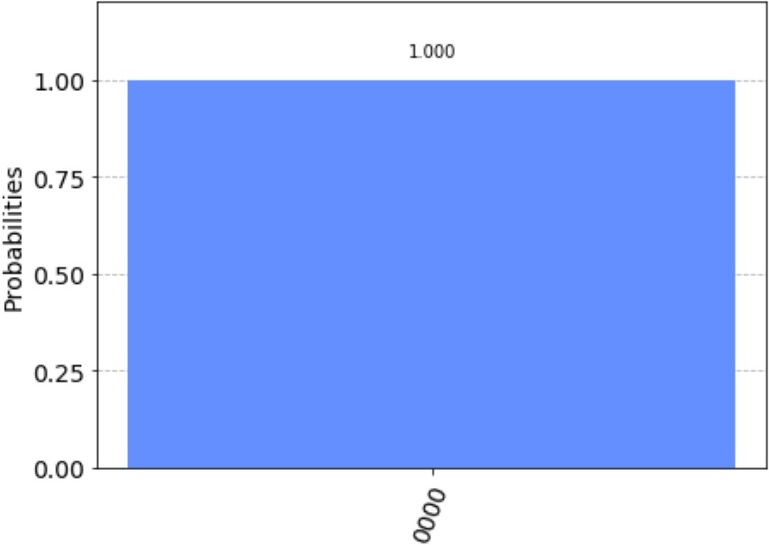
\includegraphics[width=1\textwidth]{images/simulator_constant}
        \caption{Resultados con función constante en simulador.}
        \label{fig:fig66}
    \end{minipage}\hfill
    \begin{minipage}{0.45\textwidth}
        \centering
        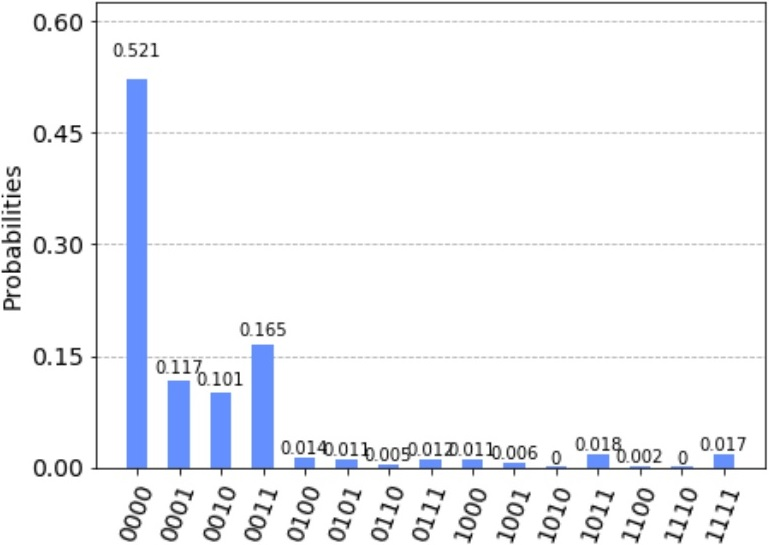
\includegraphics[width=1\textwidth]{images/ibmq_constant}
        \caption{Resultados con función constante en ordenador cuántico de IBM.}
        \label{fig:fig67}
    \end{minipage}
\end{figure}

\section{Otros algoritmos cuánticos}
\label{sec:sec62}

A continuación, vamos a presentar  dos de los algoritmos más notables en el campo. Lo haremos de forma breve debido a la dificultad para exponerlos en profundidad en un número de páginas reducido y a los límites de páginas recomendado para esta memoria.

En primer lugar tenemos el \textit{algoritmo de búsqueda de Grover} [\cite{grover1996fast}]. La búsqueda en una lista desordenada de $N$ elementos por medio de un algoritmo clásico tiene coste $\orden{N}$, mientras que el algoritmo de Grover tiene coste $\orden{\sqrt{N}}$. Para simplificar tomaremos $N$ como una potencia de $2$ tal que $N=2^n$. El algoritmo procede a codificar las entradas mediante $n$ qubits haciendo uso del paralelismo cuántico logrando el estado $\ket{s}=\frac{1}{\sqrt{2^n}}\sum_{i=0}^{2^n-1}\ket{i}$. A continuación, debemos hacer uso de una transformación cuántica, que denotamos $U_f$ y denominamos \textit{oráculo}, de manera que actúa sobre la entrada que buscamos, que denotamos $w$, tal que $U_f\ket{x}=-\ket{x}$ si $x=w$ y $U_f\ket{x}=\ket{x}$ en otro caso. Evidentemente, la transformación $U_f$ depende de la lista y su construcción no tiene por qué ser trivial. Tras esta transformación aplicamos la denominada \textit{inversión sobre la media} $U_s=2\ket{s}\bra{s}-I$. Podemos interpretar esta transformación a nivel geométrico como una reflexión sobre la media de las amplitudes del estado resultante $U_f\ket{s}$ en el paso anterior que, por la negación del estado $\ket w$, ahora es inferior a $\frac{1}{\sqrt{2^n}}$. Si denotamos a dicha media por $M$, los estados negados que buscamos tendrán ahora una amplitud $M + |M -(-\frac{1}{\sqrt{2^n}})|$, mientras que el resto tendrán amplitudes de $M - |M -\frac{1}{\sqrt{2^n}}|$. Esto hace que se incremente la amplitud del estado $\ket w$ y decrezcan el resto. Repitiendo las transformaciones $U_fU_s$ en el orden de $\orden{\sqrt{N}}$ sobre el estado inicial $\ket s$ obtenemos que $\left(U_fU_s\right)^{\sqrt{N}}\ket{s}\approx\ket w$.

Concluimos el capítulo con el también ya mencionado algoritmo de Shor [\cite{shor1994algorithms}]. Inspirado en el trabajo desarrollado por Daniel Simon que, sin embargo, fue publicado más tarde [\cite{simon1997power}]. Logra factorizar un entero de $n$ cifras en tiempo polinómico, mientras que los mejores algoritmos clásicos tienen coste exponencial sobre el número de cifras. Este algoritmo combina computación clásica y cuántica y se basa en el hecho conocido de que dado un entero $N$ a factorizar, éste tiene factores comunes con $a^{\frac{q}{2}}+1$ o $a^{\frac{q}{2}}-1$, obtenibles fácilmente gracias al máximo común divisor y donde $a$ es un entero aleatorio no factor de $N$ y menor que $N$ y $q$ es el periodo de la función $f(x)=a^x\modulo N$, que debe ser par (si no debemos escoger otro entero $a$). Si $q$ es el periodo de la función tenemos que $a^q=1\modulo N$ y por ser par tenemos que $a^q-1=(a^\frac{q}{2}+1)(a^\frac{q}{2}-1)=0\modulo N$. Si ninguno son múltiplos de $N$ (si no volvemos a repetir la elección de $a$) tienen que tener factores no triviales en común con $N$.

En el caso del algoritmo de Shor, el uso de la computación cuántica se da exclusivamente en el cálculo del periodo para lo que se usa la \textit{transformada cuántica de Fourier}, la versión análoga de la transformada de Fourier clásica y que también es usada en otros famosos algoritmos cuánticos como el de \textit{estimación de fase} [\cite[221-225]{nielsen2001quantum}].